
%%%%%%%%%%%%%%%%%%%%%%%%%%%%%%%%%%%%%%%%%%%%%%%%%%%%%%%%%%%%%
\subsubsection{具体分析}

问题一要求建立入口条件（温度$T_{in}$、入口浓度$C_{in}$、流量$Q$）与操作参数（各电场二次电压$U_i$、振打周期$T_i$）对出口粉尘浓度$C_{out}$的定量关系模型，并重点研究振打周期对瞬时排放峰值的影响规律，属于机理建模与因果分析类问题。

对历史数据执行预处理与特征统计分析，发现$C_{out}$标准差仅$0.17$且数据最大值被限制为$50.00\ \text{mg/Nm}^3$，系传感器量程限幅所致，纯数据驱动回归外推不可靠；据此以Deutsch方程等物理机理模型为主框架，从历史数据拟合待定系数；同步建立电耗—电压关系模型与振打瞬时峰值半经验估算公式；并以随机森林特征重要性交叉验证机理模型识别的主导因素。

具体分析流程如图\ref{fig:analysis1_flow}所示。

\begin{figure}[H]
  \begin{center}
    \begin{tikzpicture}[x=1cm, y=0.7cm]
      \node[box] (n11) at (0, 0) {数据预处理};
      \node[box] (n12) at (5, 0) {特征统计};
      \node[box] (n13) at (10, 0) {电耗模型};
      \node[box] (n22) at (5, -3) {Deutsch拟合};
      \node[box] (n21) at (0, -3) {振打衰减};
      \node[box] (n23) at (10, -3) {峰值估算};
      \node[box] (n31) at (0, -6) {特征重要性};
      \node[box] (n32) at (5, -6) {交叉验证};
      \node[box] (n33) at (10, -6) {结果汇总};
      \draw[arrow] (n11) -- (n12);
      \draw[arrow] (n12) -- (n13);
      \draw[arrow] (n23) -- (n22);
      \draw[arrow] (n22) -- (n21);
      \draw[arrow] (n13) -- ++(0,-1.0) -| (n23);
      \draw[arrow] (n21) -- (n31);
      \draw[arrow] (n31) -- (n32);
      \draw[arrow] (n32) -- (n33);
    \end{tikzpicture}
    \caption{问题一分析流程图}
    \label{fig:analysis1_flow}
  \end{center}
\end{figure}

% ============================================================
\subsubsection{模型准备}

在进行建模之前，需对原始数据预处理并确定建模路线。

原始数据来源于附件\texttt{Cement\_ESP\_Data.csv}，含$10080$条分钟级记录与$14$个字段（时间戳、$T_{in}$、$C_{in}$、$Q$、$U_{1\sim4}$、$T_{1\sim4}$、$C_{out}$、$P_{total}$）。

经检查发现：（1）$C_{out}$存在$50$个缺失值；（2）$C_{out}$历史标准差仅$0.17$，集中在$49.89\pm0.17$范围内，数据最大值被限制为$50.00$，系传感器量程限幅的典型特征；（3）前后电场参数差异显著——$U_1,U_2\approx58\ \text{kV}$而$U_3,U_4\approx48\ \text{kV}$，$T_1,T_2\approx230\ \text{s}$而$T_3,T_4\approx441\ \text{s}$，不可混用统一边界。

针对上述问题，预处理步骤如下：
（1）对$C_{out}$的$50$个缺失值采用时间线性插补，即$\hat{C}_{out}(t) = C_{out}(t_1) + \frac{C_{out}(t_2) - C_{out}(t_1)}{t_2 - t_1}(t - t_1)$，以保持时序局部连续性。
（2）对每个字段按$3\sigma$准则标记异常值（$|x-\mu|>3\sigma$），只标记不丢弃，异常信息供后续引用。
（3）各电场独立统计参数边界：电压上限预留$20\%$外推裕度（$U_{max,i}=1.2\times\max(U_i)$，变压器允许短时过载20\%），振打周期取$95$分位数作为安全上限$T_{crit,i}$。

图\ref{fig:ts_input}和图\ref{fig:ts_output}展示了除尘器连续7天的运行时序，半透明色带标注了K-Means工况划分结果（R0--R5，详见5.2节）。可以直观观察到入口浓度$C_{in}$和温度$T_{in}$存在显著的日周期波动，而$C_{out}$始终被限制在$50\;\text{mg/Nm}^3$附近。

\begin{figure}[H]
  \centering
  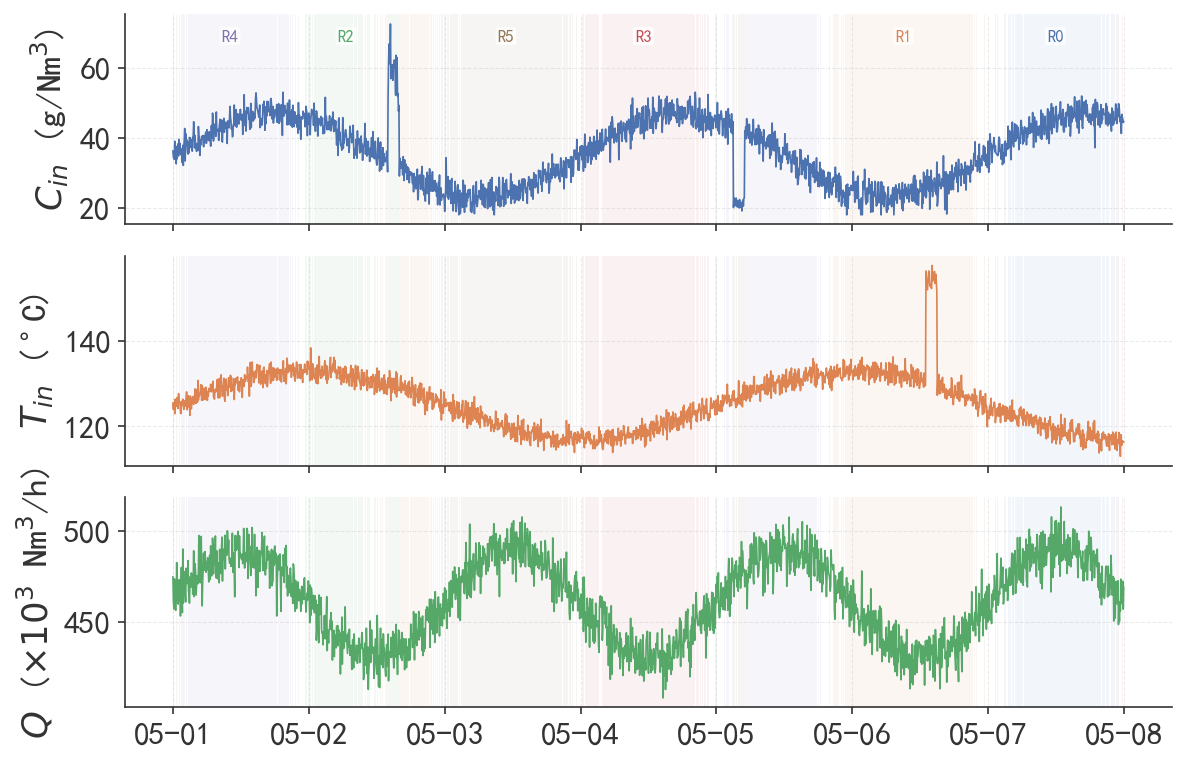
\includegraphics[width=\textwidth]{figures/timeseries_input.png}
  \caption{7天入口工况时序与工况划分}
  \label{fig:ts_input}
\end{figure}

\begin{figure}[H]
  \centering
  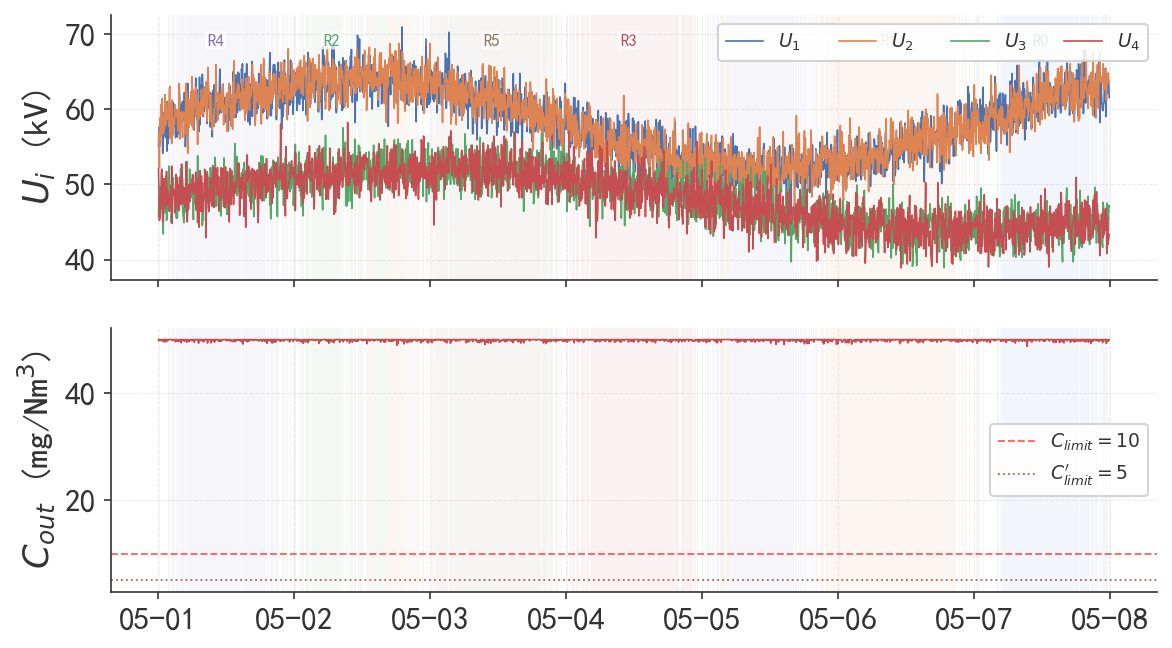
\includegraphics[width=\textwidth]{figures/timeseries_output.png}
  \caption{7天操作参数与出口浓度时序}
  \label{fig:ts_output}
\end{figure}

预处理后，数据规模为$10080$行$\times14$列，各电场边界统计如表\ref{tab:bounds}所示。

\begin{table}[H]
  \centering
  \caption{各电场参数边界统计}
  \begin{tabularx}{\textwidth}{CCCCCCC}
    \toprule
    电场 & $U_{min}$ (kV) & $U_{max}$ (kV) & $T_{min}$ (s) & $T_{max}$ (s) & $T_{crit}$ (s) & $T_{ref}$ (s) \\
    \midrule
    1 & 55.0 & 69.6 & 180 & 300 & 287 & 233 \\
    2 & 55.0 & 69.6 & 180 & 300 & 287 & 233 \\
    3 & 45.0 & 57.6 & 300 & 600 & 570 & 445 \\
    4 & 45.0 & 57.6 & 300 & 600 & 570 & 445 \\
    \bottomrule
  \end{tabularx}
  \label{tab:bounds}
\end{table}

\textbf{建模路线决策。}$C_{out}$方差仅$0.17$且数据最大值被限制为$50$，若用纯数据驱动回归（随机森林、神经网络）学习"操作参数如何降低$C_{out}$"，因变量几乎不变，模型学到的梯度接近零，外推到$C_{out}\leq10$甚至$\leq5$的区域完全不可靠。因此确定以Deutsch方程等物理机理模型为主框架，从历史数据只拟合其中的待定系数；外推时靠物理单调性约束保证趋势合理；数据驱动模型仅用于特征重要性的交叉验证，不作为外推依据。

综上所述，数据预处理完成，建模路线确定为"机理为主、数据驱动为辅"，为后续建模提供了清洁的输入数据与明确的策略方向。
